\chapter[Background]{Background} \label{ch:background}

In this chapter, we describe the key concepts that are necessary to understand
the studies that are performed in this thesis.

\section{Issue Reports}

One of the main factors that drives software evolution is the issues that are
filed by users, developers, and quality assurance personnel. Below, we describe
what issues are and the major steps involved in addressing and integrating them.

We use the term {\em issue} to broadly refer to bug reports, enhancements, and
new feature requests~\cite{giuliano2008}.  Issues can be filed by users,
developers, or quality assurance personnel. To track development progress,
software teams may use an ITS such as
Bugzilla\smartfoot{\url{https://www.bugzilla.org}} or
JIRA.\smartfoot{\url{https://www.atlassian.com/software/jira}} Such ITSs allow
for describing and monitoring the state of the issue reports.

Each issue in an ITS has a unique identifier, a brief description of the nature
of the issue, and a variety of other meta-data. Large software projects receive
plenty of issue reports on a daily basis. For example, the Eclipse and Firefox
projects respectively received an average of 65 and 89 issue reports daily (from
January to October 2016) on their
ITSs.\smartfoot{\url{https://bugs.eclipse.org/bugs}}$^,$\smartfoot{\url{https://bugzilla.mozilla.org/}}
The number of filed issues is usually greater than the size of the development
team. 

\begin{figure}[t]
	\centering
	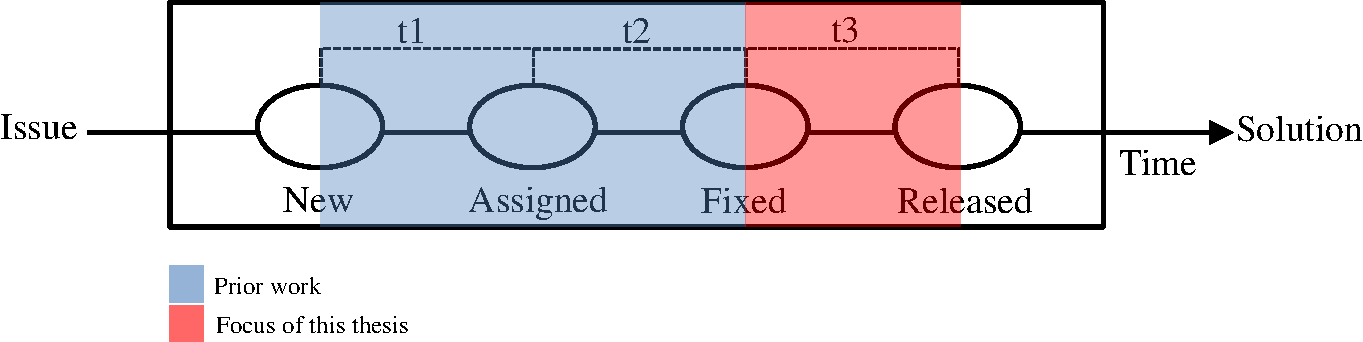
\includegraphics[width=\textwidth,keepaspectratio]
	{chapters/chapter2/figures/issue_lifecycle.pdf}
	\caption{An overview of an issue's life cycle.}
	\label{fig:issue_lifecycle2}
\end{figure}

\hyperref[fig:issue_lifecycle2]{Figure}~\ref{fig:issue_lifecycle2} shows the
stages of an issue's life cycle. After an issue has been filed, project managers
and team leaders {\em triage} them, \ie assign them to developers, denoting the
urgency of the issue using priority and severity fields~\cite{Anvik2006} (time
{\em t1} of \hyperref[fig:issue_lifecycle2]{Figure}~\ref{fig:issue_lifecycle2}). 

After being triaged, issues are then {\em addressed} (or {\em fixed} in case of
bugs), \ie solutions to the described issues are provided by developers (time
{\em t2} of \hyperref[fig:issue_lifecycle2]{Figure}~\ref{fig:issue_lifecycle2}).  Generally speaking, an issue may be in an open or closed state.  An
issue is marked as open when a solution has not yet been found. We consider
UNCONFIRMED, CONFIRMED, and IN\_PROGRESS as open states. An issue is considered
closed when a solution has been found. 

Usually, a \textit{resolution} is provided with a closed issue. For instance, if
a developer made code changes to address an issue, the state and resolution
combination should be RESOLVED-FIXED.  However, if the developer was not able to
reproduce the bug, then the state and resolution may be
RESOLVED-WORKSFORME.\smartfoot{\url{https://bugzilla.mozilla.org/page.cgi?id=fields.html}}

Finally, addressed issues must be integrated into an official release (\ie
releases that are intended for end users) in order to make them available (time
{\em t3} of \hyperref[fig:issue_lifecycle2]{Figure}~\ref{fig:issue_lifecycle2}),
which is the life cycle stage that is mainly studied in this thesis.  The life
cycle of issues is documented in detail on the Bugzilla
website.\smartfoot{\url{https://bugzilla.readthedocs.org/en/5.0/using/editing.html\#life-cycle-of-a-bug}}
In the next sections, we describe the stages of the life cycle of an issue.

\conclusionbox{Prior work studied the triaging and fixing time of issues (blue
	color in
	\hyperref[fig:issue_lifecycle2]{Figure}~\ref{fig:issue_lifecycle2}). The
	focus of this thesis is the study of the delivery delay (red color in
	\hyperref[fig:issue_lifecycle2]{Figure}~\ref{fig:issue_lifecycle2}),
which is the needed time to deliver issues that are already addressed.}

\section{Triaging Issues}

{\em Issue triaging} is the process of deciding which issues have to be
addressed and assigning the appropriate developer to them \cite{Anvik2006}. This
decision depends of several factors, such as the impact of the issue on the
software or how much effort is required to address the issue.  Projects receive
a high number of issue reports, which is usually larger than the developer team.
Hence, effective triaging of issue reports is an important means of keeping up
with user demands. 

Hooimeijer and Weimer \cite{Hooimeijer2007} built a model to classify whether or
not an issue report will be ``cheap'' or ``expensive'' to triage by measuring
the quality of the report. Based on their findings, the authors state that the
effort required to maintain a software system could be reduced by filtering out
reports that are ``expensive'' to triage. Saha \etal \cite{Saha2014} studied
long lived issues, \ie issues that were not addressed for more than one year.
They found that the time to assign a developer and address such issues is
approximately two years. Our research complements these prior studies by
investigating the time that is necessary to deliver addressed issues 
rather than the time that is necessary to triage issues.

\section{Addressing Issues}
Once an issue is properly triaged, the assigned developer starts to address it.
To estimate the required time
to address issues, some approaches used the similarity of an issue report to
prior issue reports~\cite{Weib2007,Zhang2013}, while others built prediction models using different machine learning
techniques~\cite{Panjer2007,Anbalagan2009,Giger2010, Marks2011}. 

Kim and Whitehead~\cite{Kim2006} computed the time that was necessary to address
issues in ArgoUML and PostgreSQL. They found that the median issue fixing time
is about 200 days. Guo \etal~\cite{Guo2010} used logistic regression model to
predict the probability that a new issue will be fixed. The authors trained the
model on Windows Vista issues and achieved a precision of 0.68 and recall of
0.64 when predicting Windows 7 issue reports. These approaches focus on
estimating the required time to address an issue. In our studies, however, we
investigate the required time to deliver issues that are already addressed.

Recent empirical studies assess the relationship between the attributes that are
used to build prediction models for estimating the fixing time of issues.
Bhattacharya and Neamtiu \cite{Bhattacharya2011} performed univariate and
multivariate regression analyses to capture the significance of four attributes
in issue reports.  Their results indicate that more independent variables are
required to build better prediction models. 

Herraiz \etal~\cite{Herraiz2008} studied the mean time to close issues that were
reported to the Eclipse project and how severity and priority levels of the
issues affect such a time. In their study, the authors used one way analysis of
variance to group the different priority and severity levels that were used in
the issue reports of the Eclipse project. Based on their results, the authors
suggest the reduction of the currently used severity and priority levels to
three levels. 

Zhang \etal \cite{Zhang2012} investigated the delays incurred by developers in
the issue addressing process. The authors extract the duration of an issue (\ie
from open to closed) using interaction logs. The authors investigated the impact
of three dimensions of attributes that are related to issues: issue report
characteristics, source code, and code changes. The authors found that
attributes such as severity, operating system, issue description, and number of
comments are likely to impact the needed time to start addressing an issue as
well as the needed time to resolve an issue. 

As Zhang \etal \cite{Zhang2012}, we use attributes that are related to issue
reports to build explanatory models.  Nevertheless, our goal is to study
attributes that share a relationship with the needed time to deliver addressed
issues. We also investigate the impact that severity and priority levels have on
the delivery delay of addressed issues. 

\section{Integrating Issues} 

After issues are addressed, they need to be integrated into an official release,
so users can be benefited from them. Usually, user-intended releases are shipped
along with release notes, which are documents that specify what was added,
changed, or removed in such new
releases.\smartfoot{\url{https://www.mozilla.org/en-US/firefox/releases/}} Prior
research has studied the integration of addressed issues.
Jiang~\etal~\cite{Jiang2013} studied the integration process of the Linux
kernel. They found that 33\% of code patches that were submitted to resolve
issues are accepted into an official Linux release after 3 to 6 months.
Choetkiertikul~\etal~\cite{riskyissues2015a,riskyissues2015b} studied the risk
of issues introducing delays to deliver new releases of a software project.  In
this thesis, our focus is on the time that is required to deliver addressed
issues rather than the process of patches acceptance or the risk of a release
schedule slippage.

\section{Delivery Delay}\label{ch2:deliverydelay}

{\em Delivery delay} refers to the time between the moment at which an issue is
addressed (\ie changed to the RESOLVED-FIXED status) to the time at which such
an addressed issue is shipped to end users. In 
\DIFdelbegin \DIFdel{our quantitative studies
(}\DIFdelend \hyperref[st:study1]{Studies}~\ref{st:study1} and~\ref{st:study3}\DIFdelbegin \DIFdel{)}\DIFdelend , we analyze
two {\em dimensions} of delivery delay. The first dimension is comprised of two
types of delivery delay, which are: {\em (i)} delivery delay in terms of number
of releases and {\em (ii)} delivery delay in terms of days. As for the second
dimension, we study the {\em (iii)} prolonged \DIFdelbegin \DIFdel{integration time}\DIFdelend \DIFaddbegin \DIFadd{delivery delays}\DIFaddend .

\begin{figure}
	\centering
	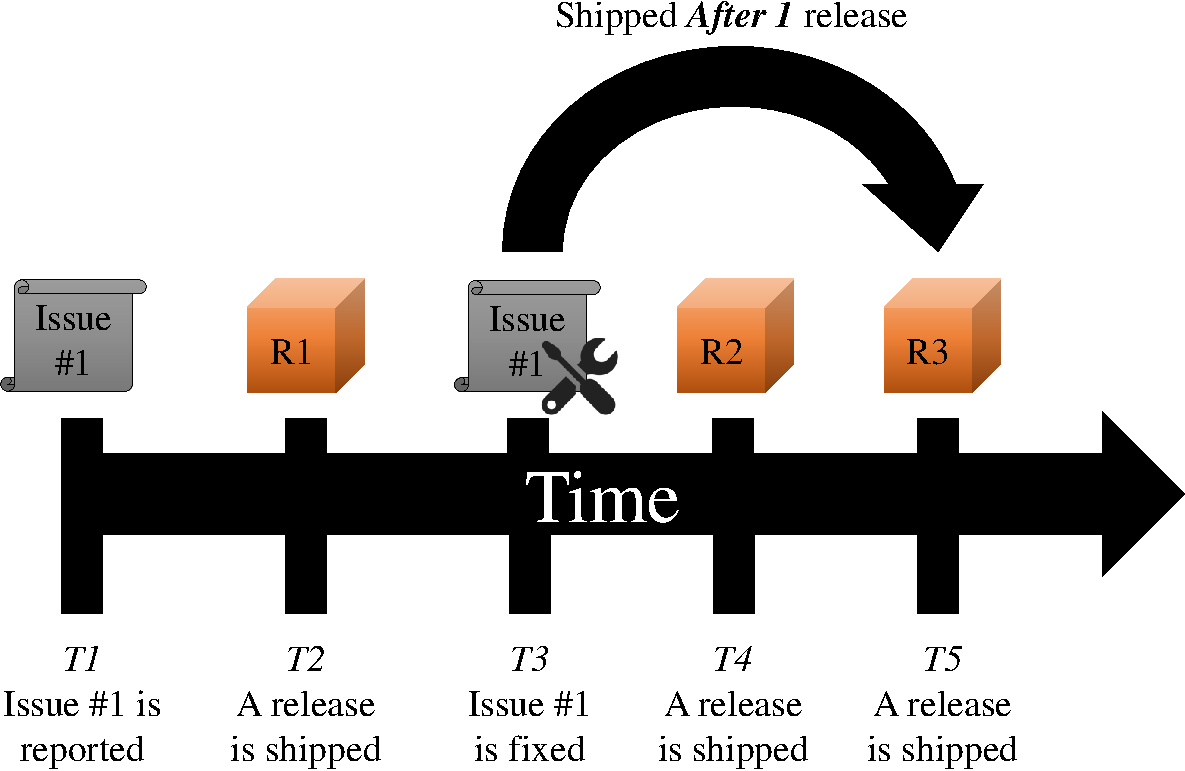
\includegraphics[width=.80\textwidth,keepaspectratio]
	{chapters/chapter2/figures/integration_delay_releases.pdf}
	\caption{An illustrative example of how we compute \DIFdelbeginFL \DIFdelFL{integration time}\DIFdelendFL \DIFaddbeginFL \DIFaddFL{delivery delays}\DIFaddendFL .}
	\label{fig:integration_delay_releases}
\end{figure}

\mydef{Delivery delay in terms of releases}{def:1}
\hyperref[fig:integration_delay_releases]{Figure}
\ref{fig:integration_delay_releases} provides an example of how we measure
delivery delay. To compute the delivery delay in terms of number of releases, we
count the number of releases that a given fixed issue is prevented from
\DIFdelbegin \DIFdel{integration}\DIFdelend \DIFaddbegin \DIFadd{delivery}\DIFaddend . In
\hyperref[fig:integration_delay_releases]{Figure}~\ref{fig:integration_delay_releases},
Issue~\#1 is reported at time~{\em $t_1$}, fixed at~{\em $t_3$}, and shipped at
time~{\em $t_5$}. The \DIFdelbegin \DIFdel{integration time }\DIFdelend \DIFaddbegin \DIFadd{delivery delay }\DIFaddend in terms of releases for Issue \#1 is the
number of official releases that are shipped between {\em $t_3$} and {\em
$t_5$}. Therefore, Issue~\#1 has a delivery delay of one release. 

\mydef{Delivery delay in terms of days}{def:2} We compute delivery delay in
terms of days using an approach that is similar
to~\hyperref[def:1]{Definition}~\ref{def:1}. However, instead of counting the
number of official releases, we count the number of days between {$t_3$} and
{$t_5$} (see
\hyperref[fig:integration_delay_releases]{Figure}~\ref{fig:integration_delay_releases}).
For instance, if the number of days between $t_i$ and $t_{(i+1)}$ in
\hyperref[fig:integration_delay_releases]{Figure}~\ref{fig:integration_delay_releases}
is 30 days, the delivery delay of issue~\#1 would be 60 days.

\mydef{Prolonged delivery delay}{def:3} Prolonged delivery delay occurs when the
delivery delay in terms of days (see \hyperref[def:2]{Definition}~\ref{def:2})
for a given addressed issue is above one {\em Median Absolute Deviation} (MAD)
of the median delivery delay of a studied project. MAD is the median of the
\textit{absolute deviations} from one distribution's median. The higher the MAD,
the greater is the variation of a distribution with respect to its
median~\cite{howell2005median,leys2013detecting}.

\section{Release Cycles} \label{subsec:firefox_releases}
\DIFdelbegin %DIFDELCMD < 

%DIFDELCMD < %%%
%DIF < \begin{figure}[t!] \centering
%DIF < 	\includegraphics[width=0.80\textwidth,keepaspectratio]
%DIF < 	{chapters/chapter2/figures/rapid-cycle-crop.pdf} \caption{Releases built
%DIF < 	into NIGHTLY channel are migrated to be stabilized into AURORA and BETA
%DIF < channels until it gets ready to be released into RELEASE channel.}
%DIF < \label{fig:rapid_cycle} \end{figure}
\DIFdelend 

A {\em release cycle} is the time period that is required by the development
team to develop and deliver a new release to end users. These releases could be
made available every few weeks or months, depending on the project release
policy. Releasing every few weeks is typically referred to as a \textit{rapid
release} cycle, while releasing monthly or yearly is typically referred to as a
\textit{traditional release} cycle~\cite{Mantyla2013}.

In our studies, we consider a release cycle length in the scale of days or weeks
as a {\em rapid} release cycle. For example, the release cycle of the Firefox
project is currently 6
weeks.\smartfoot{\url{https://wiki.mozilla.org/Release_Management/Release_Process}}
On the other hand, we consider a release cycle length of  several months or
years (\eg 12-18 months) as a traditional release cycle. In
\hyperref[st:study3]{Study}~\ref{st:study3}, we study the impact of adopting a
rapid release cycle on the delivery delay of addressed issues.

\section{Chapter Summary}

In this chapter, we provide the key concepts that we use in our studies to the
reader. We first present the concept of an {\em issue report}, which can either
represent an enhancement, a new feature, or a bug that has to be addressed in a
given project. Next, we describe the life cycle of an issue, which is basically
comprised of the {\em triaging}, {\em addressing}, and {\em integration} stages.
We then define the various types of {\em delivery delay} that we study in this
thesis. Finally, we describe the two types of release cycles that are
investigated in this thesis, which are the {\em rapid} and {\em traditional}
release cycles.

